\begin{problem}{빛의 전사 크리퓨어}{표준 입력(stdin)}{표준 출력(stdout)}{1\,초}{1024\,MB}


여기는 평화로운 알고리즘 나라. 알고리즘 나라의 외곽에는 원 모양의 울타리가 쳐져 있다.

원 둘레에는 같은 간격으로 $L$개의 기둥이 세워져 있고, 각 기둥은 $0$번부터 $L-1$번까지 시계방향 순으로 번호가 부여된 상태이다. 즉 $0$번 기둥의 시계방향에는 $1$번 기둥이 이웃해 있고, 반시계방향으로 $L-1$번 기둥이 이웃해 있다. ($L$은 홀수)

편의상 $0$번 기둥이 12시 방향에 위치하도록 회전시킨 상태로 생각하자.

\begin{figure}[h]
    \centering
    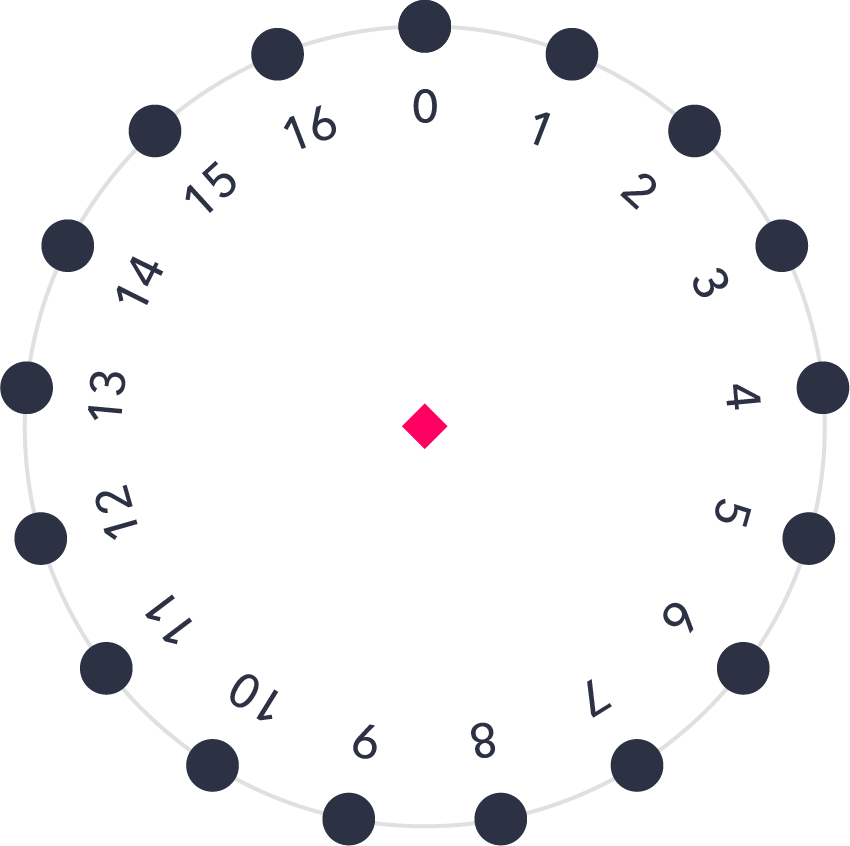
\includegraphics[width=0.25\textwidth]{../pictures/fig1.png}
\end{figure}

알고리즘 나라에는 나라의 수호자 크리퓨어가 살고 있다. 그 어떤 악인도 크리퓨어를 보게 되면 ``\texttt{그저 빛...}" 을 외치며 마음이 깨끗하게 정화된다. 때문에 이 마을에서는 그를 빛의 전사 $ \color{red}{크} \color{orange}{리} \color{blue}{퓨} \color{teal}{어} $라고 부르고, :fan: 클럽 등을 운영하며 그를 찬양하고 있다.

오늘은 알고리즘 나라에서 UCPC 2020 본선 대회가 열리는 날. 평화롭게 UCPC 대회를 진행하던 어느 순간, 사악한 악당 pichulia가 알고리즘 나라를 습격했다! 평소 알고리즘 나라에 악감정이 있던 pichulia는 기둥간에 $N$개의 고무줄을 연결하는 장난을 쳤다. pichulia가 설치한 $N$개의 고무줄 중 하나라도 남아 있으면 \textsf{\color{red}{출력\,초과}}를 받게 되므로, 이들을 모두 끊어내야 한다.

\begin{figure}[h]
    \centering
    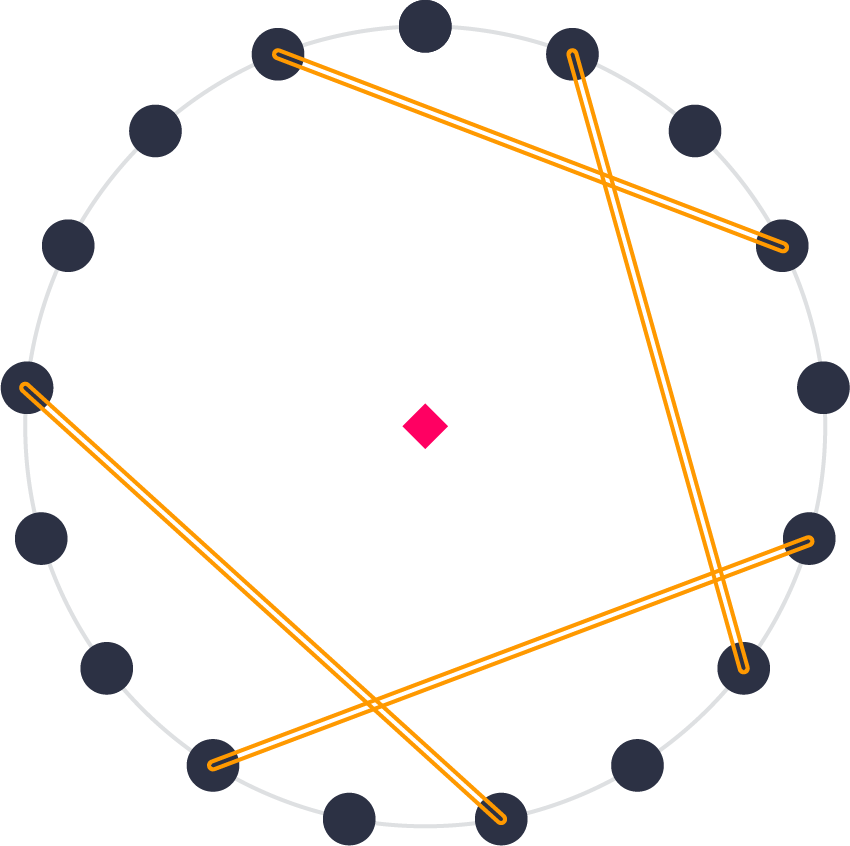
\includegraphics[width=0.25\textwidth]{../pictures/fig2.png}
\end{figure}

알고리즘 나라의 수호자 크리퓨어는 이러한 장난을 그냥 두고 볼 수 없었다. 따라서 크리퓨어의 필살기인 $\color{red}{루비빔}$을 발사해서 모든 고무줄을 끊어내고자 한다.

크리퓨어의 위치는 원의 중심에 있으며, 원의 중심에서 이동하지 않고 고정된 상태로 루비빔을 발사한다. 루비빔은 원의 중심에서 시작하는 반직선 형태로 표현할 수 있다. 이 반직선과 교차하면 빔에 맞은 것으로 취급되고, 빔에 한 번이라도 맞은 고무줄은 끊어진다. 고무줄을 고정시킨 기둥에 빔을 맞은 경우도 고무줄이 끊어진다. 빔의 두께와 고무줄의 두께는 무시할 수 있을 정도로 얇다.

\begin{figure}[h]
    \centering
    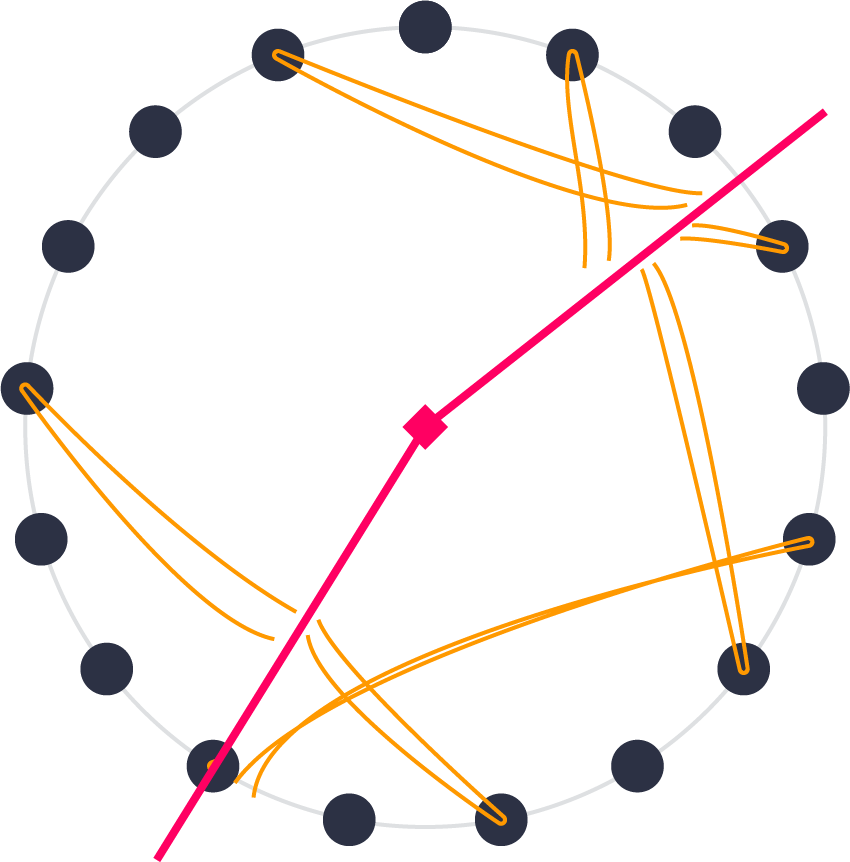
\includegraphics[width=0.25\textwidth]{../pictures/fig3.png}
\end{figure}

루비빔은 한 번 발사하는데 생각보다 많은 체력을 요구한다. 따라서 루비빔을 최소한으로 발사하는 것이 좋다.

고무줄을 모두 끊어내기 위해 필요한 루비빔 발사 횟수의 최소값을 구해서 $ \color{red}{크} \color{orange}{리} \color{blue}{퓨} \color{teal}{어} $에게 알려주자!


\InputFile
첫 번째 줄에는 $2$개의 정수 $N$과 $L$이 공백을 사이에 두고 주어진다. $N$은 고무줄의 개수이고 $L$은 원에 있는 기둥의 개수이다.
($1\leq N\leq 10^5$, $3\leq L\leq 10^9$, $L$ 은 홀수)

그 후 두 번째 줄부터 $N+1$번째 줄까지 $N$줄에 걸쳐서 고무줄의 정보를 나타내는 $2$개의 정수 $s$, $e$가 공백을 사이에 두고 주어진다. 이는 $s$번 기둥과 $e$번 기둥을 연결하는 고무줄을 설치했음을 의미한다. ($0\leq s,e\leq L-1$, $s\neq e$) 두 개 이상의 고무줄이 서로 교차할 수 있다.

$L$은 홀수이므로, 원의 중심을 지나는 고무줄은 존재하지 않는다.

\OutputFile
$N$개의 고무줄을 모두 끊어내기 위해 필요한 루비빔의 최소 발사 횟수를 출력한다.

\Examples

\begin{example}
\exmp{
4 17
3 16
1 6
10 5
8 13
}{%
2
}%
\exmp{
5 13
10 2
12 0
0 12
1 10
2 9
}{%
1
}%
\exmp{
7 27
9 3
21 2
23 7
1 3
25 7
2 18
23 18
}{%
2
}%
\exmp{
3 3
0 1
1 2
2 0
}{%
2
}%
\end{example}

\end{problem}
